\documentclass[a4paper,11pt]{article}

\usepackage[
  margin=2cm,
  bindingoffset=6mm,
  twoside
]{geometry}
\usepackage[italian]{babel}
\usepackage[utf8]{inputenc}
\usepackage[T1]{fontenc}
\usepackage{lmodern}

\usepackage{float}
\usepackage{graphics}
\usepackage{rotating}
\usepackage{enumerate}
\usepackage{booktabs}

\title{Relazione progetto}
\author{Alexandru Gabriel Bradatan}
\date{\today}

\begin{document}

\begin{titlepage}
    \begin{center}
        
\includegraphics[width=0.4\textwidth]{img/polimi-logo.png}

        \vspace*{3cm}

        \Huge
        \textbf{Relazione della prova finale di Reti Logiche}

        \vspace{1cm}

        \Large
        Alexandru Gabriel Bradatan \\
        \large
        Codice persona: 10658858 \\
        Docente di riferimento: Prof. Fornaciari \\
        Data: \today

        \vfill

        \normalsize
        a.a 2021-2022
    \end{center}
\end{titlepage}

\tableofcontents

\section{Introduzione}

Il progetto consiste nella realizzazione di un componente hardware descritto in
VHDL che dato uno stream di byte in input gli applica il codice convoluzionale
$1/2$ e restituisce uno stream in output.

\paragraph{Modello di memoria}
Il modulo si interfaccerà con una memoria RAM con 16 bit di address space,
indirizzata al byte. La memoria, non implementata all'interno del componente,
comunicherà tramite il seguente protocollo:

\begin{itemize}
  \item Un segnale di enable \texttt{mem\_en} attiverà la memoria.
  \item La modalità di accesso verrà determinata dal segnale \texttt{mem\_we}: 0
    per indicare la lettura e 1 la scrittura.
  \item L'indirizzo di lettura/scrittura viene impostato tramite il il vettore
    \texttt{mem\_address}.
  \item Nel caso di una scrittura, verranno salvati i dati presenti  in
    \texttt{mem\_in}; nel caso di una lettura, il risultato dell'operazione sarà
    disponibile in \texttt{mem\_out}.
\end{itemize}

I dati saranno distribuiti in RAM seguendo la seguente convenzione:

\begin{itemize}
  \item All'indirizzo 0 sarà salvata la lunghezza totale in byte dello stream in
    ingresso. Ciò implica che la lunghezza massima dell'input sarà di 255 byte.
  \item Nel range di indirizzi $[1;255]$ sarà salvato l'input stream
  \item Nel range di indirizzi $[1000; 65535]$ sarà salvato l'output
    dell'elaborazione.
\end{itemize}

\section{Architettura}

Il componente è suddiviso in due entità: il datapath e la macchina a stati
che governa l'elaborazione.

\subsection{Datapath}

Il datapath è suddiviso in 3 gruppi funzionali interconnessi che si occupano
ognuno di un aspetto dell'elaborazione: elaborazione di un byte, generazione del
segnale di fine elaborazione dell'input e generazione dei segnali che gestiscono
l'accesso alla memoria. Lo schema completo del datapath è riportato in
figura~\ref{fig:datapath}, ciascun modulo verrà affrontato nel dettaglio nella
sua sezione corrispondente.

\begin{sidewaysfigure}[p]
  \centering
  \scalebox{0.3}{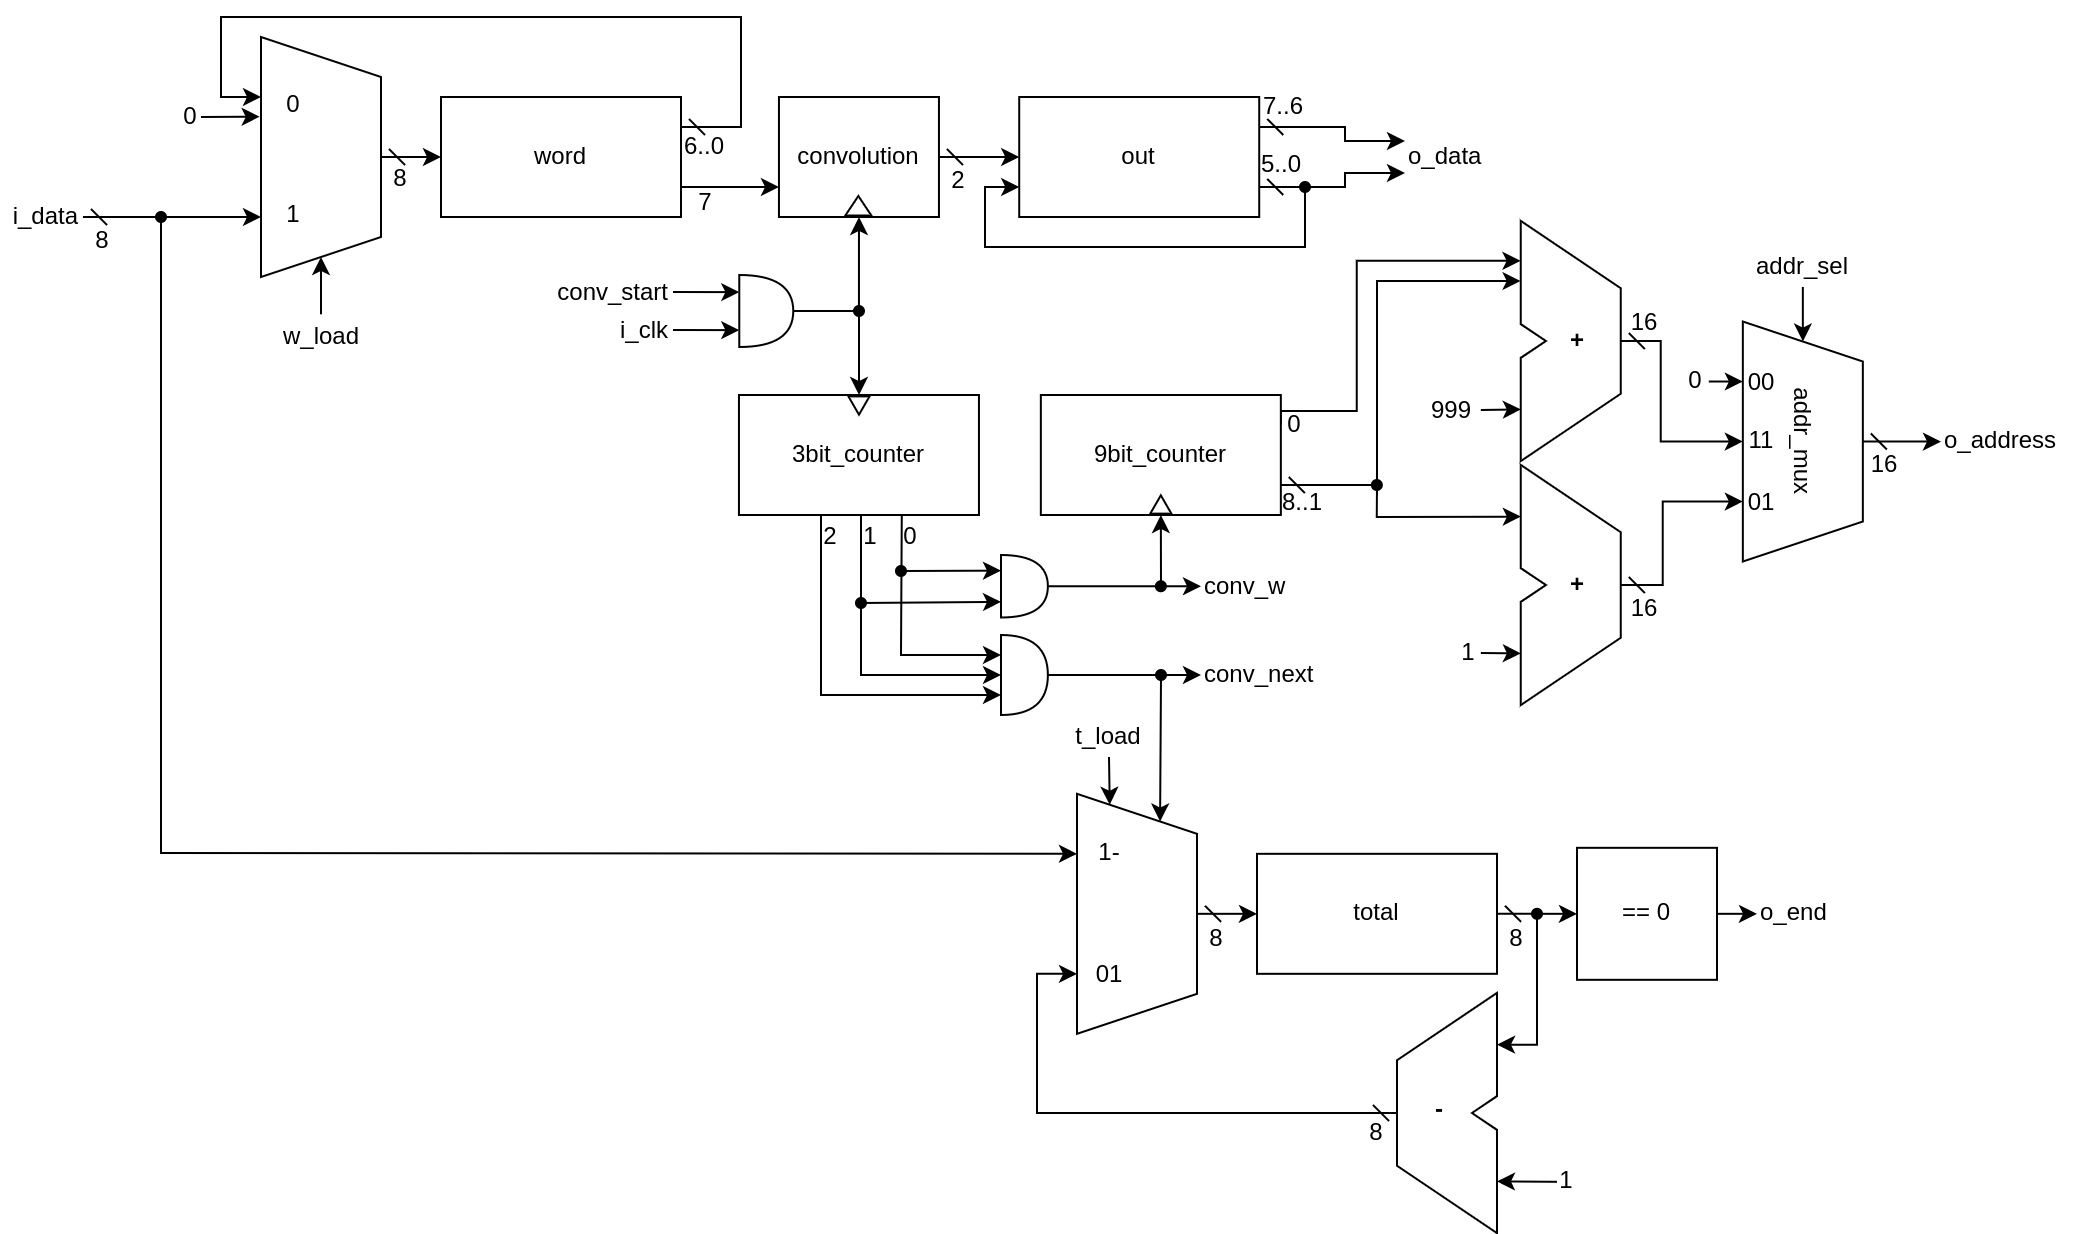
\includegraphics{./diagrams/datapath.png}}
  \caption{Schematica completa del datapath}%
  \label{fig:datapath}
\end{sidewaysfigure}

Nel suo complesso, il datapath esporrà verso la macchina a stati che lo governa
la seguente interfaccia:

\begin{itemize}
  \item \texttt{i\_clk} (in): Segnale di clock (passthrough dalla macchina a
    stati).
  \item \texttt{i\_rst} (in): Segnale di reset (passthrough dalla macchina a
    stati).
  \item \texttt{i\_data} (in): Byte letto dalla RAM (passthrough dalla macchina a
    stati).
  \item \texttt{addr\_sel} (in): Vettore di 2 bit di selezione tra 3 indirizzi. Il
    valore viene così interpretato:
    \begin{itemize}
      \item \texttt{00} si riferisce all'indirizzo 0
      \item \texttt{01} si riferisce all'indirizzo di un byte nel range $[1;
        \mathit{input\_length}]$ con $\mathit{input\_length}$ la lunghezza in
        byte dello stream in input
      \item \texttt{11} si riferisce all'indirizzo di un byte nel range $[999;
        999 + 2\mathit{input\_length}]$.
    \end{itemize}

    Gli indirizzi prodotti tramite \texttt{01} e \texttt{11} corrispondono
    rispettivamente al byte corrente in lettura e a quello corrente in
    scrittura.
  \item \texttt{t\_load} (in): Segnale di enable per il registro che salverà la
    lunghezza totale dello stream in input.
  \item \texttt{w\_load} (in): Segnale di enable per il registro che salverà la
    parola fornita in ingresso tramite \texttt{i\_data}.
  \item \texttt{conv\_start} (in): Segnale di enable per il processo di
    elaborazione di un byte.
  \item \texttt{conv\_rst} (in): Segnale di reset secondario generato dalla
    macchina a stati.
  \item \texttt{conv\_w} (out): Segnale che indica alla macchina a stati che un
    byte è pronto per la scrittura in RAM.
  \item \texttt{conv\_next} (out): Segnale che indica alla macchina a stati che
    l'elaborazione di un byte è terminata.
  \item \texttt{o\_address} (out): Vettore di 16 bit che contiene l'indirizzo
    generato tramite \texttt{addr\_sel}.
  \item \texttt{o\_end} (out): Segnale che indica la fine dell'elaborazione
    dello stream in input.
  \item \texttt{o\_data} (out): Byte da scrivere in RAM.
\end{itemize}

Ogni componente sequenziale del datapath, ad esclusione di dove indicato
diversamente, riceverà in ingresso come clock \texttt{i\_clk} e come segnale di
reset $\mathtt{i\_rst} + \mathtt{conv\_rst}$.

\subsubsection{Elaborazione di un byte}

Il processo di convoluzione può essere visto come una macchina a stati che
prende in ingresso un bit dello stream in entrata e ne produce due in uscita. La
macchina a stati è rappresentata in figura~\ref{fig:convolution-fsm}. Lo stream
in uscita avrà, quindi, il doppio della lunghezza rispetto allo stream in
entrata.

\begin{figure}[htb]
  \centering
  \scalebox{.30}{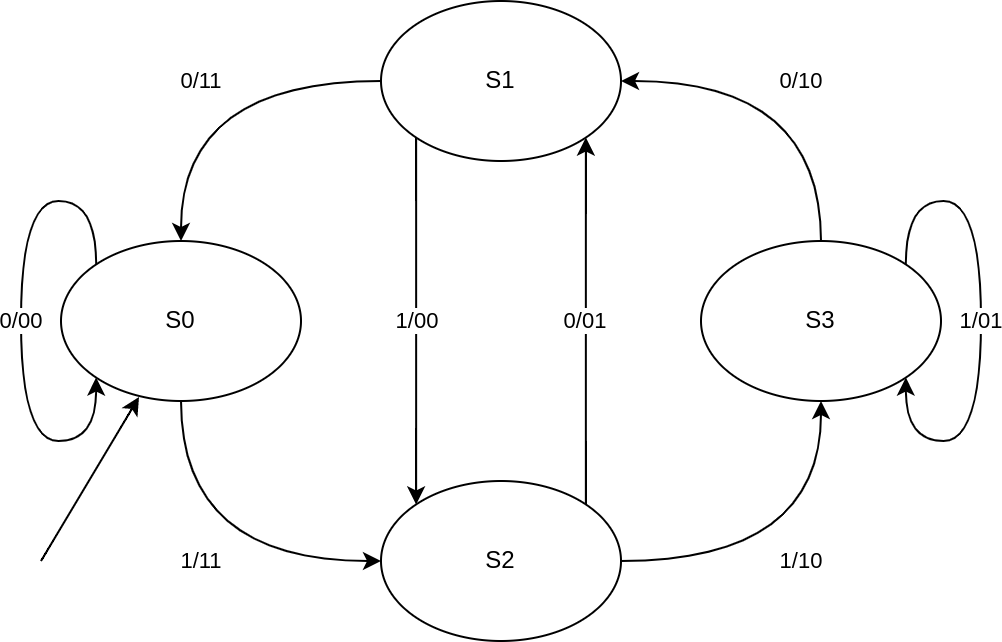
\includegraphics{./diagrams/convolution-fsm.png}}
  \caption{Macchina di Mealey rappresentante il processo di convoluzione di un byte}%
  \label{fig:convolution-fsm}
\end{figure}

\begin{figure}[htb]
  \centering
  \scalebox{0.3}{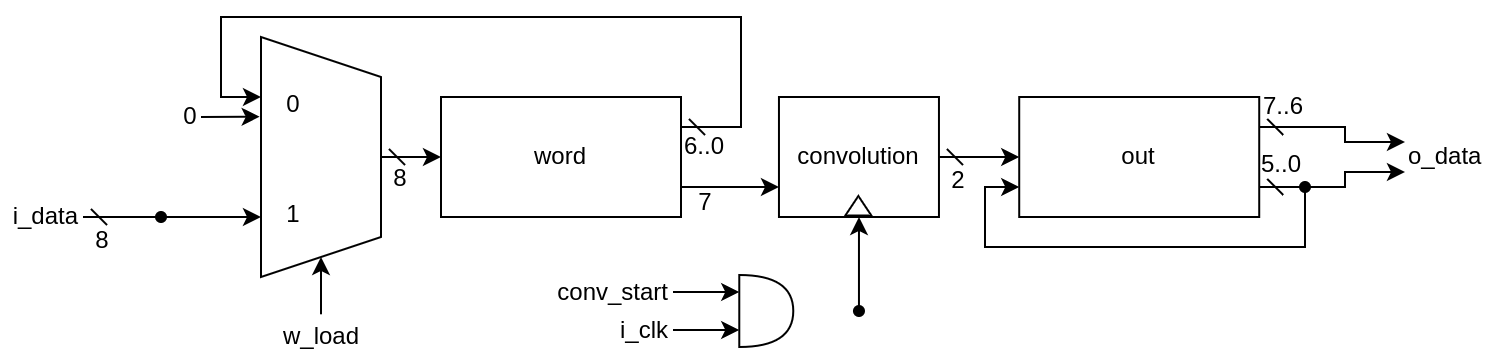
\includegraphics{./diagrams/byte-processing.png}}
  \caption{Modulo di elaborazione di un byte}%
  \label{fig:byte-processing-rtl}
\end{figure}

La rete di elaborazione è invece rappresentata in
figura~\ref{fig:byte-processing-rtl}. Il byte letto dalla RAM viene salvato in
uno shift register R-to-L a 8 bit governato dal segnale \texttt{w\_load}. Ad
ogni ciclo di clock, il MSB viene fornito alla macchina a stato di convoluzione.
L'output della convoluzione viene salvato nei 2 bit più bassi di un altro shift
register R-to-L a 8 bit (per convenzione ordiniamo i bit in ordine discendente
da sinistra a destra). Il byte da scrivere in RAM \texttt{o\_data} è composto
dalla lettura dei bit in parallelo dell'ultimo shift register. La macchina a
stati di convoluzione riceve come clock
$\texttt{conv\_start}\times\texttt{i\_clk}$.

\subsubsection{Gestione della memoria}

Il modulo di gestione della memoria è responsabile della generazione dei segnali
\texttt{o\_address}, \texttt{conv\_w} e \texttt{conv\_next}. La schematica del
modulo è riportata in figura~\ref{fig:memory-management-rtl}

\begin{figure}[htb]
  \centering
  \scalebox{0.3}{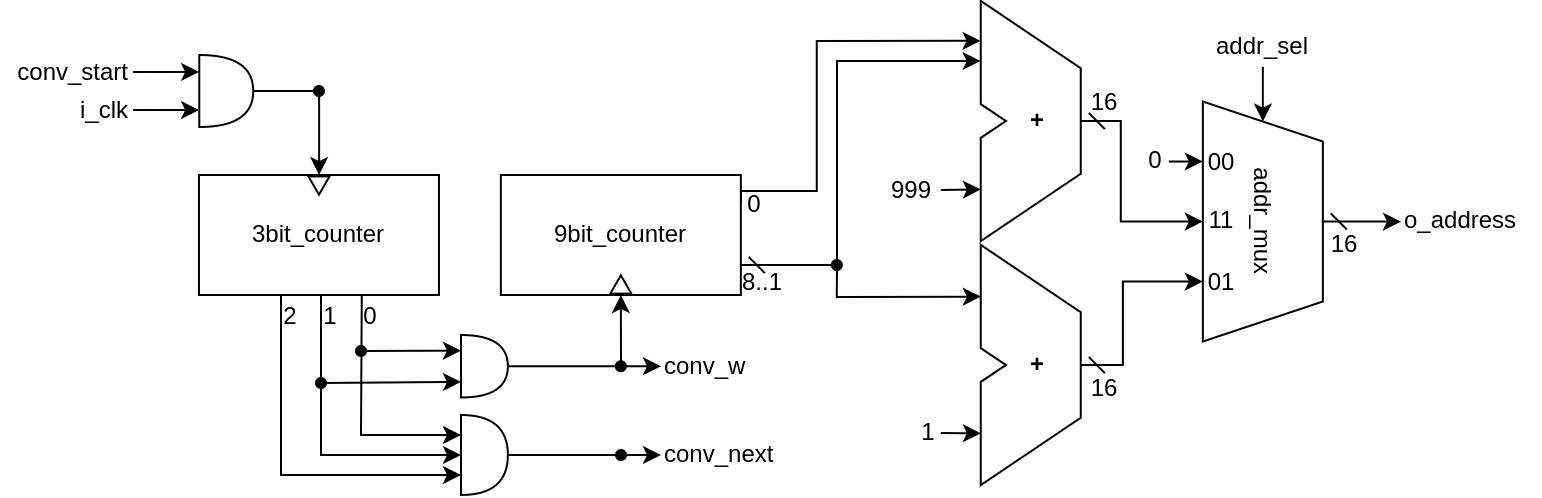
\includegraphics{./diagrams/memory-management.png}}
  \caption{Modulo di gestione della memoria}%
  \label{fig:memory-management-rtl}
\end{figure}

Il modulo utilizza due contatori, uno a 3 bit e uno a 9 bit. Il primo viene
incrementato per ogni ciclo di clock in cui la macchina di convoluzione lavora.
Esso conta il numero di coppie prodotte:

\begin{itemize}
  \item Per 4 coppie (3) il segnale \texttt{conv\_w} viene alzato
  \item Per 8 coppie (7) il segnale \texttt{conv\_next} viene alzato
\end{itemize}

Il secondo contatore conta invece i byte scritti in memoria. Poiché i dati in
uscita hanno il doppio della lunghezza di quelli in entrata, possiamo
riutilizzare lo stesso contatore per gestire sia l'indirizzo di lettura che
quello di scrittura:

\begin{itemize}
  \item Tutti i 9 bit vengono utilizzati per calcolare l'indirizzo di scrittura
  \item Gli 8 bit più significativi vengono utilizzati per calcolare l'indirizzo
    di lettura
\end{itemize}

Il valore del secondo contatore viene infine sommato a degli offset e passato al
multiplexer di selezione dell'indirizzo.

\subsubsection{Generazione del segnale di fine elaborazione}

Il modulo di generazione del segnale di fine elaborazione genera il segnale
\texttt{o\_end}. La schematica è rappresentata in
figura~\ref{fig:end-generation-rtl}.

\begin{figure}[htb]
  \centering
  \scalebox{0.3}{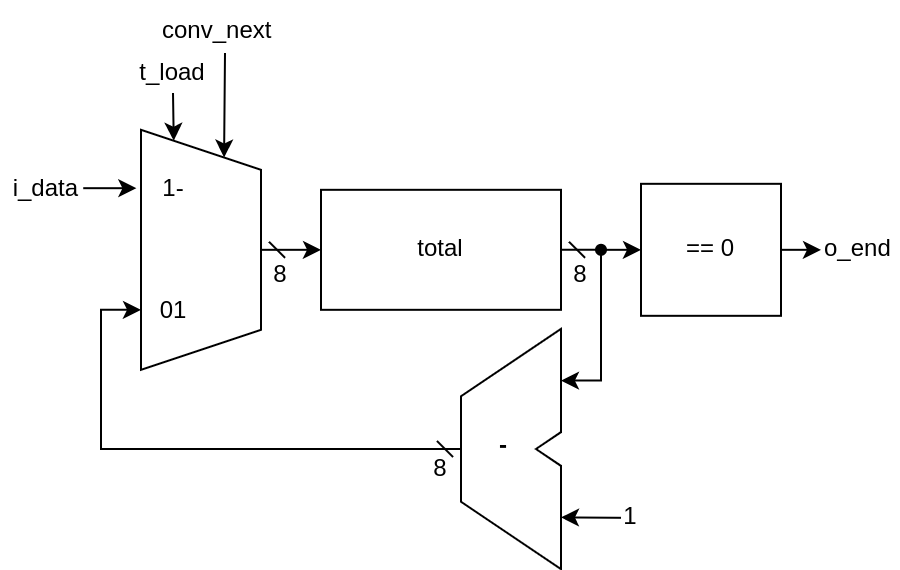
\includegraphics{./diagrams/end-generation.png}}
  \caption{Modulo di generazione del segnale di fine}%
  \label{fig:end-generation-rtl}
\end{figure}

Esso è composto da un contatore con preload in cui viene caricato ad inizio
elaborazione la lunghezza dello stream in entrata. Il valore salvato viene
decrementato ogni volta che \texttt{conv\_next} è alto. Il segnale di
\texttt{o\_end} viene impostato a 1 quando il valore salvato all'interno del
contatore è pari a 0.

\subsection{Macchina a stati}

La macchina a stati che governa il datapath è una macchina di Mealey che
espone ai morsetti i seguenti segnali:

\begin{itemize}
  \item \texttt{i\_clk} (in): Segnale di clock.
  \item \texttt{i\_rst} (in): Segnale di reset.
  \item \texttt{i\_start} (in): Segnale di inizio elaborazione
  \item \texttt{i\_data} (in): Byte letto dalla RAM.
  \item \texttt{o\_address} (out): Vettore di 16 bit che contiene l'indirizzo
    di lettura/scrittura in RAM (passthrough da datapath).
  \item \texttt{o\_done} (out): Segnale di fine elaborazione
  \item \texttt{o\_en} (out): Segnale di enable della RAM
  \item \texttt{o\_we} (out): Segnale write-enable della RAM
  \item \texttt{o\_data} (out): Byte da scrivere in RAM (passthrough da
    datapath).
\end{itemize}

Una diagramma ad alto livello della macchina a stati è presente in
figura~\ref{fig:fsm-simplified}. Il diagramma completo invece è riportato in
figura~\ref{fig:fsm}.

\begin{figure}[htb]
  \centering
  \scalebox{0.225}{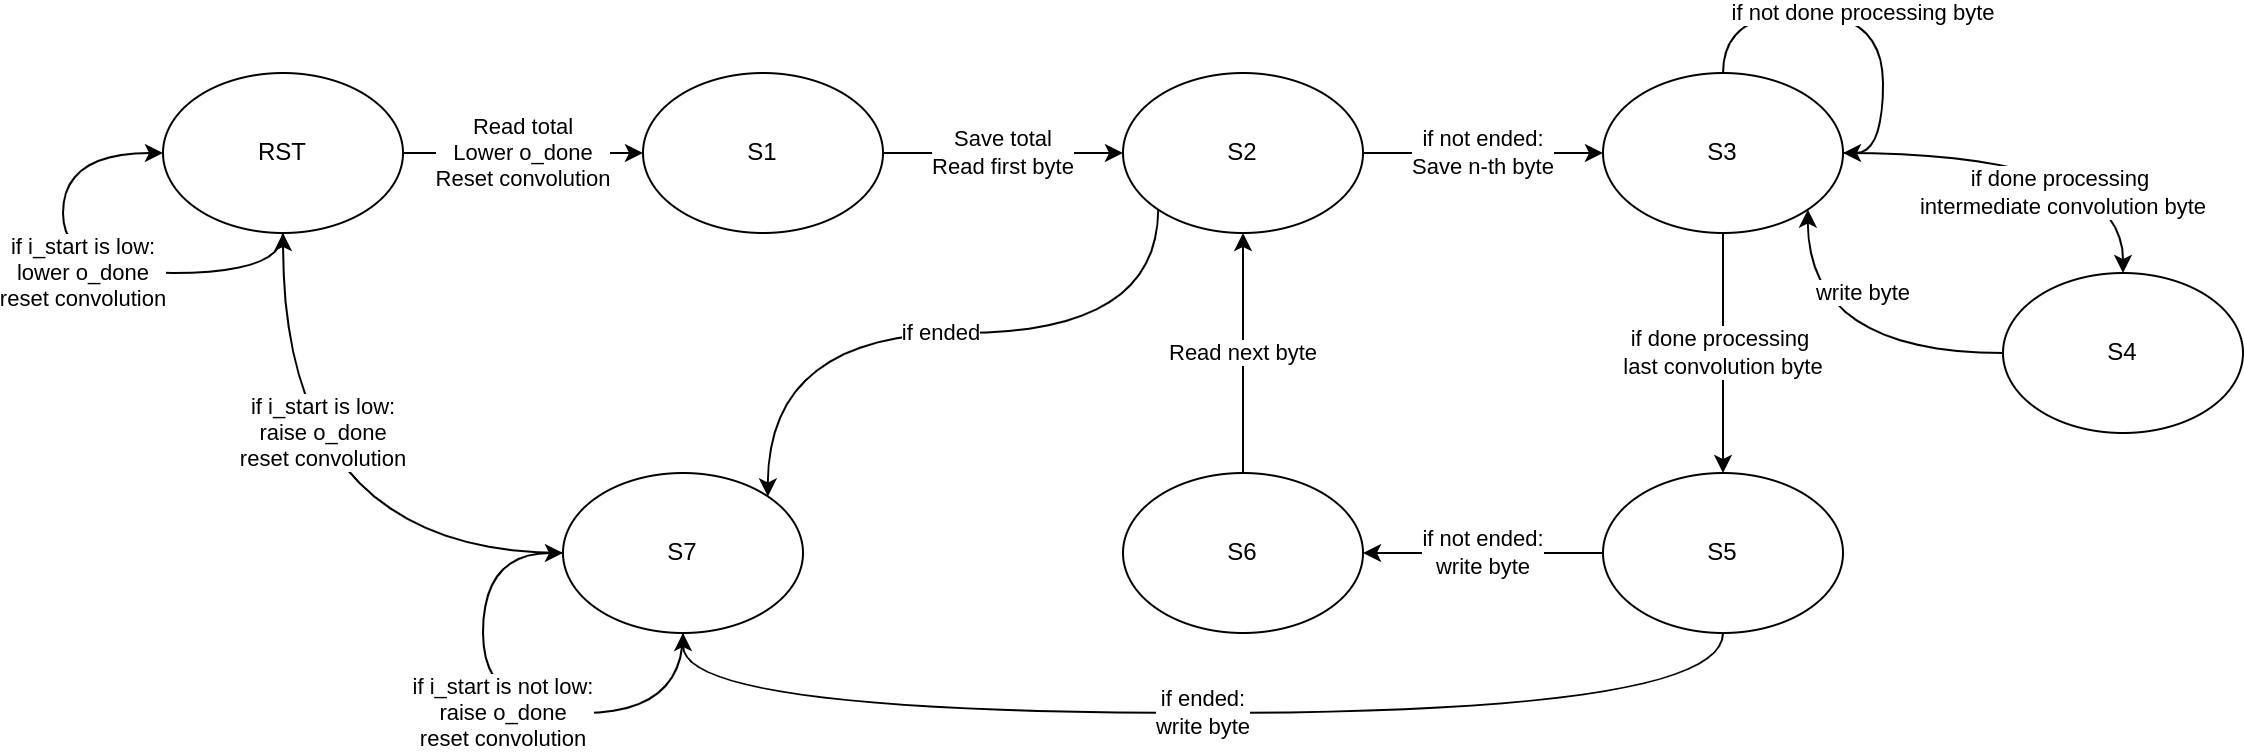
\includegraphics{./diagrams/state-machine-simplified.png}}
  \caption{Macchina di Mealey che controlla il datapath (semplificata)}%
  \label{fig:fsm-simplified}
\end{figure}

\begin{sidewaysfigure}[p]
  \centering
  \scalebox{0.3}{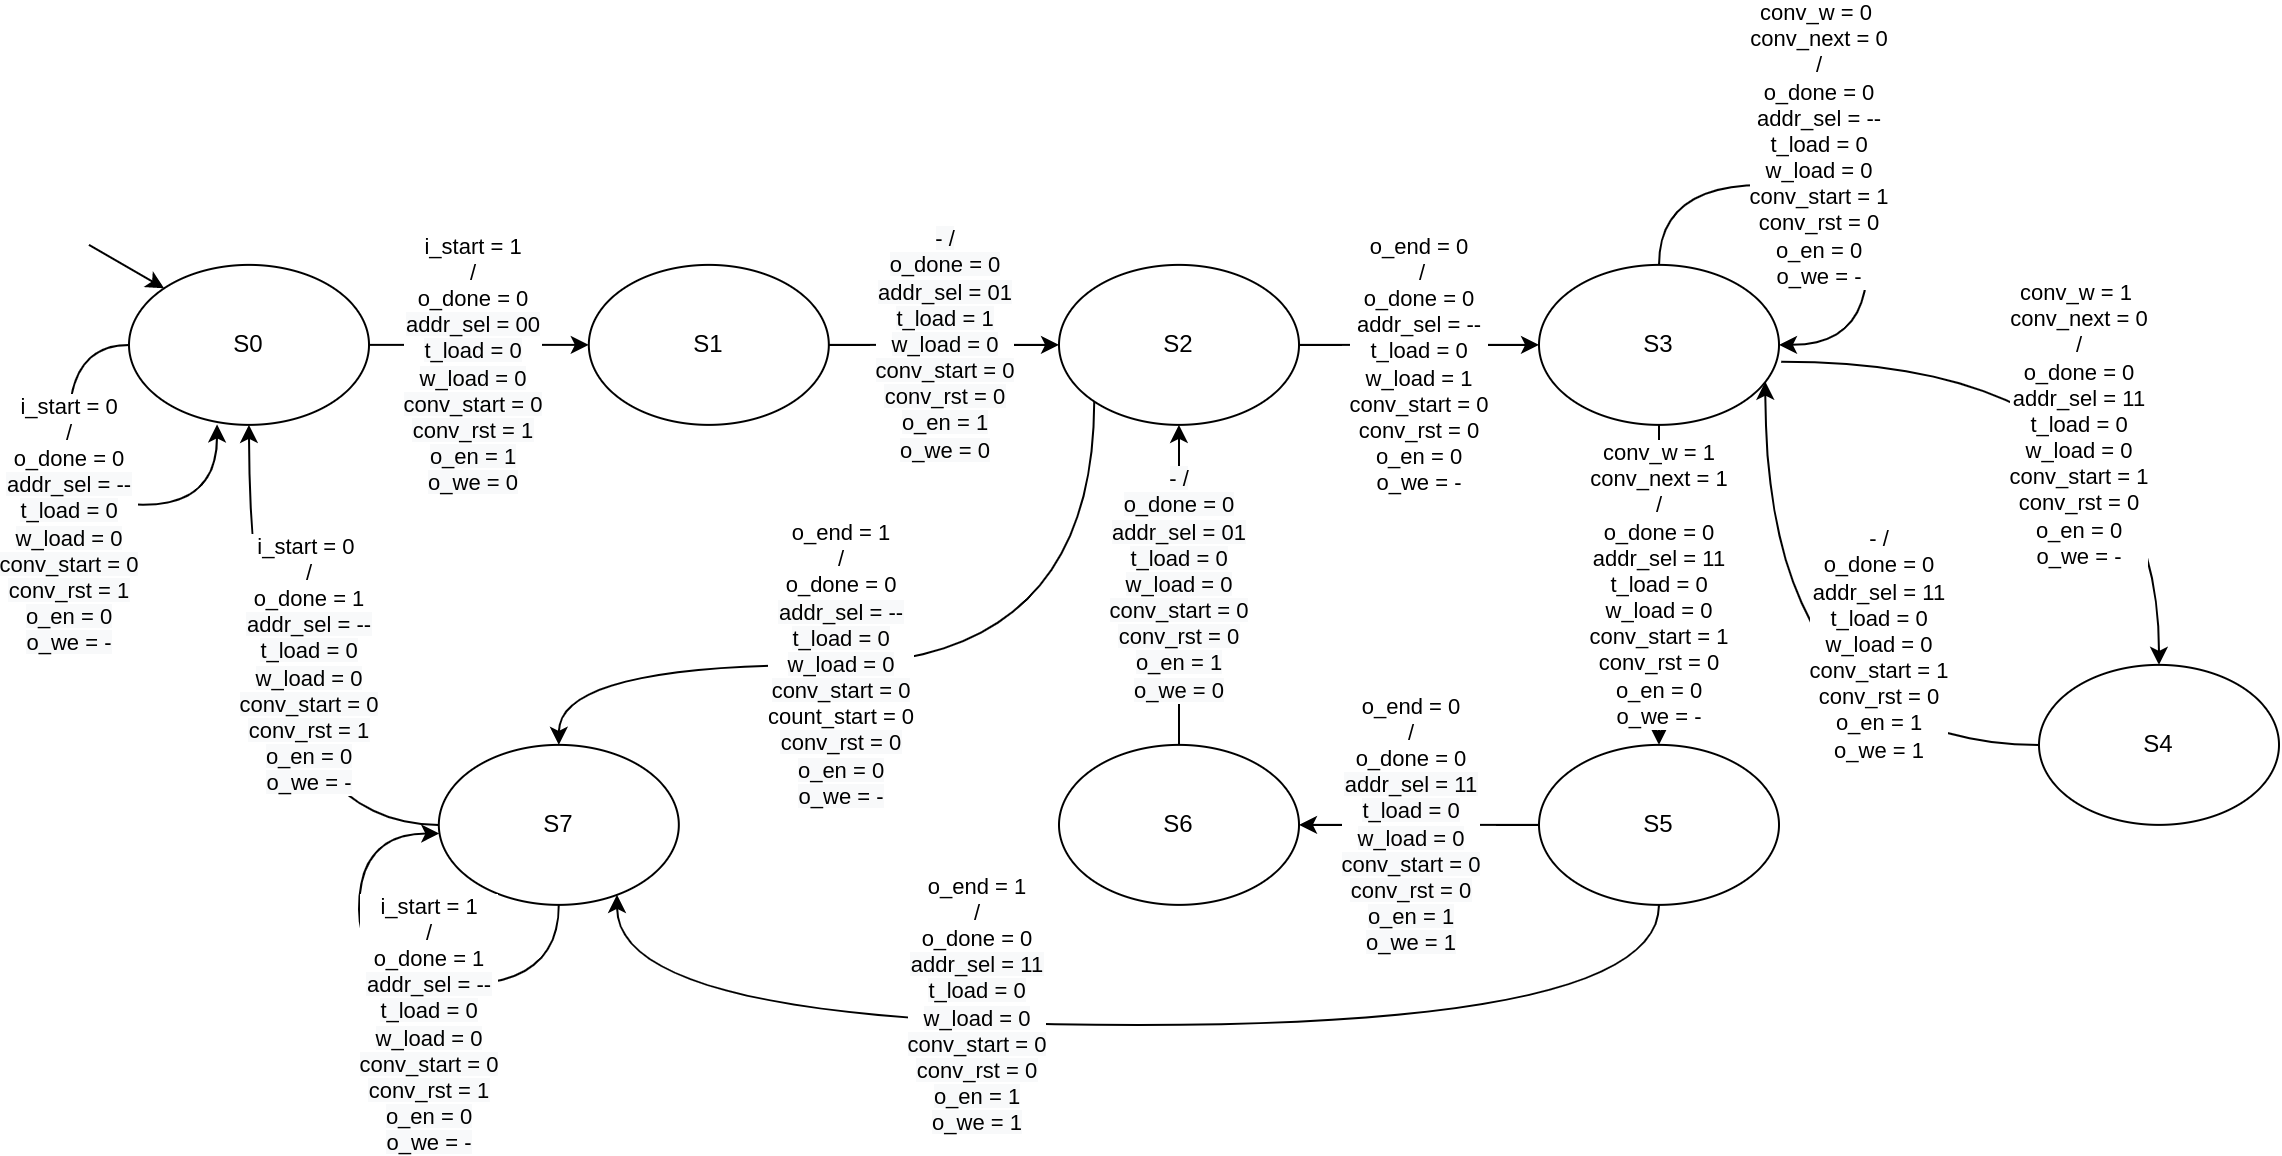
\includegraphics{./diagrams/state-machine.png}}
  \caption{Macchina di Mealey che controlla il datapath (completa)}%
  \label{fig:fsm}
\end{sidewaysfigure}

\section{Test effettuati}

Sono stati usati due testbench, ognuno dei due in grado di leggere ed eseguire
i casi di test da file. La differenza tra i due moduli sta nella modalità di
reset tra vari test-case: uno usa la funzionalità di restart che il circuito
deve implementare come per specifica, l'altro usa il segnale di RESET
\texttt{i\_rst}.

I casi limite testati sono stati:

\begin{enumerate}
  \item Lunghezza dell'input pari a 0
  \item Lunghezza dell'input diversa da 0
  \item Restart/reset tra sequenze diverse
  \item Restart/reset tra sequenze uguali
\end{enumerate}

Tutti i test sono stati eseguiti in modalità \textit{behavioural} e
\textit{functional post-synthesis}. I file letti dai testbench sono stati
scritti tramite un generatore di test scritto in python dal sottoscritto.

\section{Report di sintesi}

Nelle tabelle~\ref{tab:report-utilization} e~\ref{tab:report-timing} sono stati
riportati i dati di sintesi più importati. È stato utilizzato Vivado 2021.2 come
software di sintesi e xc7a200tfbg484-1 come FPGA di riferimento.

\begin{table}[H]
  \centering
  \begin{tabular}{c c c c}
    \toprule
    Site type & Used & Available & Utilization\% \\
    \midrule
    LUT as Logic          & 53 & 134600 & 0.04 \\
    LUT as Memory         & 0  & 134600 & 0.00 \\
    Register as Flip Flop & 41 & 269200 & 0.02 \\
    Register as Latch     & 0  & 269200 & 0.00 \\
    F7 Muxes              & 0  & 67300  & 0.00 \\
    F8 Muxes              & 0  & 33650  & 0.00 \\
    \bottomrule
  \end{tabular}
  \caption{Alcune metriche del report di utilizzo come riportato da \texttt{report\_utilization}}%
  \label{tab:report-utilization}
\end{table}

\begin{table}[H]
  \centering
  \begin{tabular}{l l}
    Slack (MET)     & \texttt{90.910ns (required time - arrival time)} \\
    Requirement     & \texttt{100.000ns (clock rise@100.000ns - clock rise@0.000ns)} \\
    Data Path Delay & \texttt{2.939ns (logic 0.999ns (33.991\%)  route 1.940ns (66.009\%))}\\
  \end{tabular}
  \caption{Alcune metriche del report di timing come riportato da \texttt{report\_timing}}%
  \label{tab:report-timing}
\end{table}

\section{Conclusione}

Si ritiene che il componente sviluppato rispetti tutti i vincoli funzionali e
non indicati nel documento di specifica.

L'architettura è stata sviluppata secondo il modello a due componenti FSM +
Datapath. Particolare attenzione è stata posta sull'efficienza: si è riuscito ad
ottenere uno slack di circa 90 nanosecondi e un utilizzo di soli 41 flip flop.
Si è inoltre evitato l'utilizzo di Latch. Alcuni dei componenti sequenziali più
complessi, come i contatori e la macchina a stati del convolutore, sono stati
specificati usando \texttt{process} per dare piena libertà al tool di sintesi di
implementarli nella maniera più efficiente.

\end{document}
